\documentclass[conference]{IEEEtran}
\IEEEoverridecommandlockouts
% The preceding line is only needed to identify funding in the first footnote. If that is unneeded, please comment it out.

%%%%%%%%%%%%%%%%%%%%%%%%%%%%%%%%%%%%%%%% Verwendete Packages
\usepackage[utf8]{inputenc} % Zeichen-Enkodierung
\usepackage[T1]{fontenc}    % Zeichen-Enkodierung
\usepackage{blindtext}      % Platzhaltertexte
\usepackage{amsmath}        % Mathematische Umgebungen und Symbole
\usepackage{algorithm}      % Umgebung für Algorithmen
\usepackage[noend]{algpseudocode} % Pseudocode innerhalb der Algorithmen
\usepackage{graphicx}       % Einbinden von Grafiken
\usepackage{xcolor}         % Farbnamen und Definition
\usepackage{subcaption}     % Subcaption für Unterabbildungen
\usepackage{array}
\usepackage{geometry}
\usepackage{hyperref} % For clickable URLs in bibliography
\usepackage{url}      % For proper formatting of URLs
\geometry{a4paper, margin=1in}
\usepackage{listings}
\lstset{
  basicstyle=\ttfamily,
  breaklines=true,     % Enables automatic line breaking
  linewidth=\linewidth % Limits the width to the current line width
}
\usepackage[acronym]{glossaries}
\makeglossaries
% \setlength{\columnsep}{0.5in}

% \usepackage[numbers,sort&compress]{natbib}

%%%%%%%%%%%%%%%%%%%%%%%%%%%%%%%%%%%%%%%% Eigene Farben definieren
\definecolor{twblue}{HTML}{1f497d}
\definecolor{structure}{HTML}{1f497d}
\definecolor{blindtext}{HTML}{D3D3D3}

\def\BibTeX{{\rm B\kern-.05em{\sc i\kern-.025em b}\kern-.08em
    T\kern-.1667em\lower.7ex\hbox{E}\kern-.125emX}}

%%%%%%%%%%%%%%%%%%%%%%%%%%%%%%%%%%%%%%%% Dokumentbeginn
\begin{document}

\title{Nonlinear Model Predictive Control-Based Local Planner with Integrated Dynamic Obstacle Avoidance for Mobile Robots}

\author{\IEEEauthorblockN{\textbf{Student:} Eppacher Kevin, BSc. \textbf{PK:} 2310331013}
        \IEEEauthorblockN{\textbf{Peer ReviewerIn:} Schwaiger Simon, MSc.}
}


\maketitle
%%%%%%%%%%%%%%%%%%%%%%%%%%%%%%%%%%%%%%%%%%%%%%%%%%%%%%%%%%%%%%%%%%

\begin{abstract}

% \title{nMPC-Local-Planner with Integrated Dynamic Obstacle Avoidance}

Mobile robots play a crucial role in various domains, including logistics and service industries, where they must navigate dynamic environments filled with fast-moving obstacles. Traditional hierarchical navigation systems separate global path planning and local obstacle avoidance, with global planners focusing on static maps and local planners using real-time sensor data for immediate adjustments. However, local planners such as DWA, TEB, and MPC struggle in highly dynamic environments due to issues such as slow responsiveness, difficulty in handling sharp turns or dense obstacles, and high computational demands, which can result in suboptimal paths or failure to avoid collisions in real time. This paper proposes a nonlinear Model Predictive Controller (nMPC) integrated with an obstacle detection algorithm to improve dynamic obstacle avoidance performance. The nMPC framework selectively extracts only the most relevant obstacles for avoidance, reducing the computational load while maintaining safety and efficiency. This optimization minimizes computation time, reduces cross-track errors, and ensures effective navigation. Through comprehensive simulations, the nMPC demonstrated superior performance compared to state-of-the-art planners in dynamic obstacle avoidance tasks, achieving faster arrival times and lower tracking errors. Future work will extend the application of this controller to real-world systems, enhancing the nMPC’s adaptability to various robotic platforms.
The project is made available on GitHub for public use and contributions at the following link: \url{https://github.com/KevinEppacher/walle\_ws.git}
\end{abstract}

\begin{IEEEkeywords}
Model Predictive Control, Differential Drive Robots, Obstacle Avoidance, Autonomous Mobile Robots, Control Algorithms
\end{IEEEkeywords}

%%%%%%%%%%%%%%%%%%%%%%%%%%%%%%%%%%%%%%%%%%%%%%%%%%%%%%%%%%%%%%%%%%
\section{Introduction}

Mobile robots are becoming increasingly indispensable in various fields such as intralogistics, public, and private services, with applications ranging from autonomous floor-cleaning robots to vacuum cleaners. In dynamic environments, these robots are frequently confronted with fast-moving obstacles, which they must detect and avoid in real-time. 

Navigation in mobile robotics is generally approached using a hierarchical paradigm, where a global planner generates a high-level path and a local planner refines this path based on real-time sensory data. The global planner operates over a static map, which is typically generated using techniques like occupancy grids, and focuses on finding an optimal or feasible path from the start to the goal location. This path is often generated by algorithms such as Dijkstra, A*, or more advanced techniques like Rapidly Exploring Random Trees (RRT) \cite{thrun2005probabilistic}.

However, the global path alone is insufficient in dynamic environments where obstacles may move or change over time. To handle these situations, the local planner operates at a higher frequency, continuously refining the robot's trajectory to avoid newly detected obstacles, while ensuring the robot still follows the general direction of the global path. The local planner relies on real-time sensory input (e.g., LiDAR or camera data) to make instantaneous adjustments, balancing both collision avoidance and adherence to the global plan \cite{khatib1986real, siegwart2011autonomous}.

This separation between global path planning, which is concerned with long-term planning over a static map, and local obstacle avoidance, which focuses on immediate reactive control, is key to ensuring that the robot can navigate effectively in both known and dynamic environments. By maintaining this hierarchical structure, robots are able to achieve long-distance navigation goals while remaining responsive to dynamic obstacles in real-time \cite{khatib1986real, siegwart2011autonomous}.


% Motivation for creating paper contribution (sehr grobe Übersicht über sota)

\cite{ASAP} conducted a comprehensive comparison of its developed local planner, ASAP, with other seminal planners, including DWA, TEB, and MPC. In \cite{ASAP}, we compare the performance of these planners in guiding a mobile robot to follow a global path while avoiding densely placed obstacles. In this study, \cite{ASAP} evaluated the local planners based on metrics such as arrival time, cross track error, and computation time. 

\begin{figure}[!h]
    \centering
    \includegraphics[width=1\columnwidth]{images/DWA_TEB_MPC_ASAP_stats.png}
    \caption{Simulation results for arrival time, cross track error and computation time for DWA, TEB, MPC and ASAP (directly taken from \cite{ASAP})}
    \label{fig:DWA_TEB_MPC_ASAP_stats}
\end{figure}

The findings in Figure \ref{fig:DWA_TEB_MPC_ASAP_stats} indicate that the MPC local planner achieved the shortest arrival time, while maintaining the same cross track error as the ASAP planner. However, when it comes to computation time, the ASAP controller was the fastest, with a processing time of just 0.2 ms, compared to DWA's 40 ms, TEB's 5 ms, and MPC's 18 ms. Furthermore, \cite{ASAP} highlights that the DWA planner had the highest collision rate, which also corresponds to its longer arrival time.

Similarly, \cite{MPCvsTEB} performed a comparison between MPC and TEB planners. The study evaluated both the TEB planner and various forms of MPC in terms of arrival time, path length, control effort, and CPU time. The results indicated that the TEB planner and the quadratic form of MPC had comparable arrival times, around 126.9 seconds. However, the time-optimal MPC, which is specifically optimized for minimizing arrival time, completed the task in just 116 seconds.

% Problem description arising from motivation (was fehlt im aktuellen sota -> vermeidung dynamischer Objekte)
Based on the findings in \cite{ASAP}, the weaknesses of the local planners DWA, TEB and MPC are highlighted, particularly in the context of dynamic obstacle avoidance.

DWA faces significant challenges when obstacles are directly in front of the robot, especially in environments with narrow passages or sharp turns. This is due to the fact that DWA samples a wide range of speeds to find a feasible collision-free trajectory, but this method increases computation time and is prone to failure in tight spaces. In addition, in environments with dynamic obstacles, velocity sampling often cannot react quickly enough, making DWA less reliable in real-time applications \cite{ASAP}.

TEB, known for generating smooth and collision-free paths, works by solving a non-convex optimisation problem. While TEB performs well in static or moderately dynamic environments, its performance degrades in highly dynamic environments due to the need for frequent re-optimisation. This can lead to suboptimal paths or deadlocks where the planner cannot find a valid solution, especially when obstacles move rapidly or unpredictably. In addition, TEB's computation time increases significantly in dense environments, further limiting its real-time applicability \cite{ASAP, MPCvsTEB}.

MPC, on the other hand, provides near-optimal trajectories by predicting future robot states and optimising control inputs based on system dynamics and constraints. However, solving these constrained optimisation problems at each time step imposes a high computational burden, especially when a longer prediction horizon is required to handle complex or dynamic environments. The real-time performance of MPC is highly dependent on the available computational resources and the complexity of the environment. Furthermore, the effectiveness of MPC is highly dependent on an accurate model of the robot and the environment, which can be difficult to achieve in real-world scenarios with unpredictable obstacles \cite{ASAP, MPCvsTEB}.

% Paper contribution
The main objective is to design a controller that effectively addresses the challenges of dynamic obstacle avoidance, offering improved performance in real-time navigation within dynamic environments. This work contributes to the State-of-the-art development, of a nonlinear Model Predictive Controller for a mobile robot with integrated dynamic sparse obstacle avoidance. This work proposed an nMPC local planner, in which the nMPC is integrated with an obstacle avoidance algorithm, to reduce computation time and increase performance, which is evaluated by reducing the arrival time and the cross-tracking error.

% The main objective is to design a local planner that effectively addresses the challenges of dynamic obstacle avoidance, offering improved performance in real-time navigation within dynamic environments.

% This work addresses these challenges by developing a nonlinear Model Predictive Controller (nMPC) for differential drive mobile robots, specifically designed for dynamic obstacle avoidance. The primary contribution is the integration of nMPC to improve real-time navigation performance in dynamic environments. Unlike conventional approaches such as DWA, the proposed nMPC effectively handles nonlinear dynamics and dynamic obstacles, offering superior prediction accuracy and responsiveness.

% This paper contributes to the field by rigorously evaluating the nMPC against both DWA and recent advancements in local planning algorithms from the past five years. The results demonstrate that the nMPC provides enhanced trajectory optimization and obstacle avoidance capabilities, filling a crucial gap in mobile robot control by addressing scenarios that existing methods have not sufficiently solved.

% Paper structure
The rest of the paper is organized as follows: Section II discusses related work in local path planning and obstacle avoidance. Section III outlines the methodology used. Section IV describes how the methods were implemented and evaluated. In Chapter IV, the results of the experiments are presented. In Chapter V, the results are discussed and critically reflected upon. Chapter VI summarizes this work and gives an outlook on future research.

%%%%%%%%%%%%%%%%%%%%%%%%%%%%%%%%%%%%%%%%%%%%%%%%%%%%%%%%%%%%%%%%%%
\section{State-of-the-Art}

This section provides an overview of several state-of-the-art local controllers, including the Dynamic Window Approach (DWA), Timed Elastic Band (TEB) and Model Predictive Control (MPC). In contrast, nonlinear Model Predictive Control (nMPC) is presented to overcome these limitations and provide improved performance.

\subsection{Preliminary Information on Optimization-Based Methods}

Optimization-based methods like DWA, TEB, and MPC solve an Optimal Control Problem (OCP) by minimizing a cost function while respecting system constraints. The cost function is an objective measure that typically balances factors such as trajectory tracking, control effort, and obstacle avoidance. Its goal is to find control inputs that minimize deviation from the desired path while maintaining safety and efficiency.

In OCPs, equality constraints ensure the system dynamics are followed, while inequality constraints handle limits such as collision avoidance and control input bounds. The problem is often discretized using methods like multiple shooting or single shooting, which transform the continuous problem into a finite-dimensional optimization problem.

These optimization problems are solved in real-time using solvers such as Quadratic Programming (QP), Interior Point Optimizer (IPOPT), or Sequential Quadratic Programming (SQP), which can handle both the constraints and optimization efficiently over the prediction horizon.

\subsection{Dynamic Window Approach (DWA)}
DWA is a popular local planner that selects safe and feasible velocities by sampling translational \((v)\) and rotational \((\omega)\) velocities within a dynamic window, reinitialising the current pose and velocities and the current obstacle position. These sampled velocities are evaluated through an objective function that balances forward movement and obstacle avoidance. DWA computes a set of trajectories and selects the one that maximizes progress toward the goal while ensuring the robot avoids collisions \cite{DWA, fox1997dynamic}.

The velocities \(v\) and \(\omega\) are constrained within bounds (see Eq. \ref{eq:dwa_constraints}):

\begin{equation}
\label{eq:dwa_constraints}
v_{min} \leq v \leq v_{max}, \quad \omega_{min} \leq \omega \leq \omega_{max}
\end{equation}

The objective function \(G(v, \omega)\) evaluates the alignment with the goal, distance to obstacles, and forward velocity (see Eq. \ref{eq:dwa_objective}):

\begin{equation}
\label{eq:dwa_objective}
G(v, \omega) = \alpha \cdot \text{heading}(v, \omega) + \beta \cdot \text{clearance}(v, \omega) + \gamma \cdot v
\end{equation}

While DWA is efficient and handles real-time obstacle avoidance well, it struggles with dynamic obstacles due to its lack of future obstacle movement prediction. The extensive velocity sampling can lead to increased computation times in complex environments \cite{DWA}.

Recent enhancements to DWA focus on improving computational efficiency and addressing the limitations in dynamic environments. A faster implementation of DWA based on non-discrete path representation \cite{lin2023faster} reduces the computational complexity by eliminating discrete path representations and employing polar coordinate transformations. Another improved version integrates reinforcement learning (RL) techniques \cite{zhou2022improved}, dynamically adjusting the sampling window size to better handle obstacles in real-time, which improves efficiency and accuracy in dynamic environments.

\subsection{Timed Elastic Band (TEB)}
TEB models the robot’s trajectory as a dynamic band that adjusts to avoid obstacles while satisfying kinodynamic constraints. The trajectory is continuously optimized using a cost function that takes into account the goal, collisions, and system dynamics \cite{inproceedings}.

The cost function \(J(\mathbf{x}, \mathbf{v})\) over the series of poses \(\mathbf{x}\) and velocities \(\mathbf{v}\) is defined in Equation \eqref{eq:teb_cost}:

\begin{equation}
\label{eq:teb_cost}
\begin{aligned}
J(\mathbf{x}, \mathbf{v}) = \sum_{i=1}^{n-1} \big( & \text{cost}_{\text{goal}}(x_i) + \text{cost}_{\text{collision}}(x_i) \\
& + \text{cost}_{\text{kinodynamics}}(v_i) \big)
\end{aligned}
\end{equation}

TEB is effective at generating smooth trajectories that adapt to obstacles and kinodynamic constraints. However, in highly dynamic environments, TEB's computational complexity can increase significantly. Additionally, its performance is sensitive to initial conditions and parameter tuning.

Recent improvements to TEB incorporate dynamic obstacle velocities using Kalman filtering to predict obstacle movement and optimize the trajectory in real time. This improved TEB method \cite{pr12050984} enhances real-time performance by reducing the overall computational burden while maintaining a high success rate for dynamic obstacle avoidance.

\subsection{Model Predictive Control (MPC)}

Model Predictive Control (MPC) computes optimal control inputs over a prediction horizon by solving an optimization problem that accounts for both system dynamics and environmental constraints. The fundamental principle of MPC is to generate a trajectory by forward-simulating the system’s dynamics over a prediction horizon, while adhering to constraints and minimizing a cost function. At each time step, the optimization problem is solved, and only the first control input is applied, making the process iterative and reactive to dynamic environments.

The optimization problem involves the system model \(x_{k+1} = f(x_k, u_k)\), where \(x_k\) represents the system state and \(u_k\) represents the control input at time step \(k\). The MPC aims to minimize the cost function \(J(\vec{x}_k, \vec{u}_k)\), as shown in Equation \eqref{eq:mpc_cost}:

\begin{equation}
\label{eq:mpc_cost}
\min_{\vec{u}_k} J(\vec{x}_k, \vec{u}_k) = \phi(\vec{x}(N)) + \sum_{k=0}^{N-1} L(\vec{x}(k), \vec{u}(k))
\end{equation}

where \( \phi(\vec{x}(N)) \) is the terminal cost, and \(L(\vec{x}(k), \vec{u}(k))\) represents the running cost over each time step \(k\). The term \( \phi(\vec{x}(N)) \) penalizes the deviation of the final state \(\vec{x}(N)\) from the desired target state, ensuring that the robot closely follows the planned trajectory by the end of the prediction horizon. The running cost \(L(\vec{x}(k), \vec{u}(k))\) is a quadratic function of both the state and the control input, where:

- \( Q \) is the state weighting matrix, which penalizes deviations of the robot’s state from the desired reference trajectory. Larger values in \( Q \) correspond to higher penalties for errors in specific state variables, such as position or velocity.

- \( R \) is the control input weighting matrix, which penalizes large or sudden control inputs. This encourages smoother and more efficient control actions, avoiding erratic behavior.

- \( S \) is the terminal cost weighting matrix, which emphasizes the importance of reaching the target state at the end of the prediction horizon, ensuring that the final state is as close as possible to the desired state. The overall objective of the cost function is to balance minimizing the tracking error while ensuring efficient use of control inputs.

Compared to DWA and TEB, MPC offers superior handling of dynamic obstacles by continuously adjusting the robot’s trajectory in real-time, optimizing for both safety and performance. Unlike DWA, which samples a range of velocities and often struggles with sharp turns or dense obstacle fields due to its reactive nature, MPC employs a predictive approach that anticipates future states, making it more adaptable to dynamic scenarios \cite{ASAP}. Additionally, while TEB excels at generating smooth paths, it frequently encounters computational challenges in complex environments, especially when faced with multiple moving obstacles. The non-convex optimization problem that TEB solves can result in suboptimal paths or deadlocks, particularly when obstacles move unpredictably \cite{ASAP, MPCvsTEB}.

MPC, on the other hand, directly integrates the system’s nonlinear dynamics and constraints into its optimization process. By predicting future states and control inputs over a finite prediction horizon, MPC is capable of generating near-optimal paths that ensure collision-free navigation, even in highly dynamic environments. An additional advantage of the nMPC controller is its ability to enforce both hard and soft constraints. The soft constraints allow for minor violations (penalizing the cost function when predicted states approach obstacles), thereby guiding the robot towards safer paths. The hard constraints, on the other hand, guarantee a strictly collision-free trajectory by setting firm limits that cannot be breached. This dual-constraint structure provides flexibility in optimization while ensuring safety \cite{wan2024MultiUAVsNMPC}.

However, one of the long-standing challenges of MPC has been its computational intensity. Solving a constrained optimization problem in real-time, especially with a large prediction horizon, demands significant computational resources \cite{MPC_ROS, Model_predictive_Controller_for_Mobile_Robot}. To overcome this challenge, a sparse obstacle representation is integrated into the proposed nMPC framework. By selectively focusing on the most relevant obstacles and discarding less critical data, the computational load is reduced, allowing for real-time performance while retaining the predictive capabilities of MPC. This integration not only lowers the computational cost but also enhances the planner’s ability to efficiently handle dynamic environments with high obstacle density \cite{Lindqvist2020MPC}.

%%%%%%%%%%%%%%%%%%%%%%%%%%%%%%%%%%%%%%%%%%%%%%%%%%%%%%%%%%%%%%%%%%
\section{Methods}

Figure \ref{fig:nMPC_Local_Planner_Diagram_2} illustrates the individual components of the nMPC local planner. The main elements are the trajectory planner, nMPC and the obstacle detection algorithm.

The trajectory planner receives the global path from a planner based on Dijkstra's search. It processes the global plan into a local plan, taking into account the number of predictions and the prediction horizon length specified by the nMPC. After the nMPC receives the reference trajectory, the robot’s current pose, and the target State, the optimizer of the nMPC calculates the optimal control signal \(\mathbf{u} = \begin{bmatrix} v & \omega \end{bmatrix}^\top\), until the target is reached.

The robot is localised in a predefined map using probabilistic localisation methods \cite{thrun2005probabilistic}. Based on the scan data from the LiDAR, the DDMR can detect obstacles. The Obstacle Detection Node filters the LiDAR data to define a search cone, reducing unnecessary computational load on the nMPC. It then sends the positions of the obstacles, along with the predefined safety radius of the obstacles, to the trajectory planner, which passes this information to the nMPC for further processing. By sending only the most relevant obstacles to the nMPC, the computational load is minimized, allowing for real-time decision-making.

\begin{figure}[!h]
    \centering
    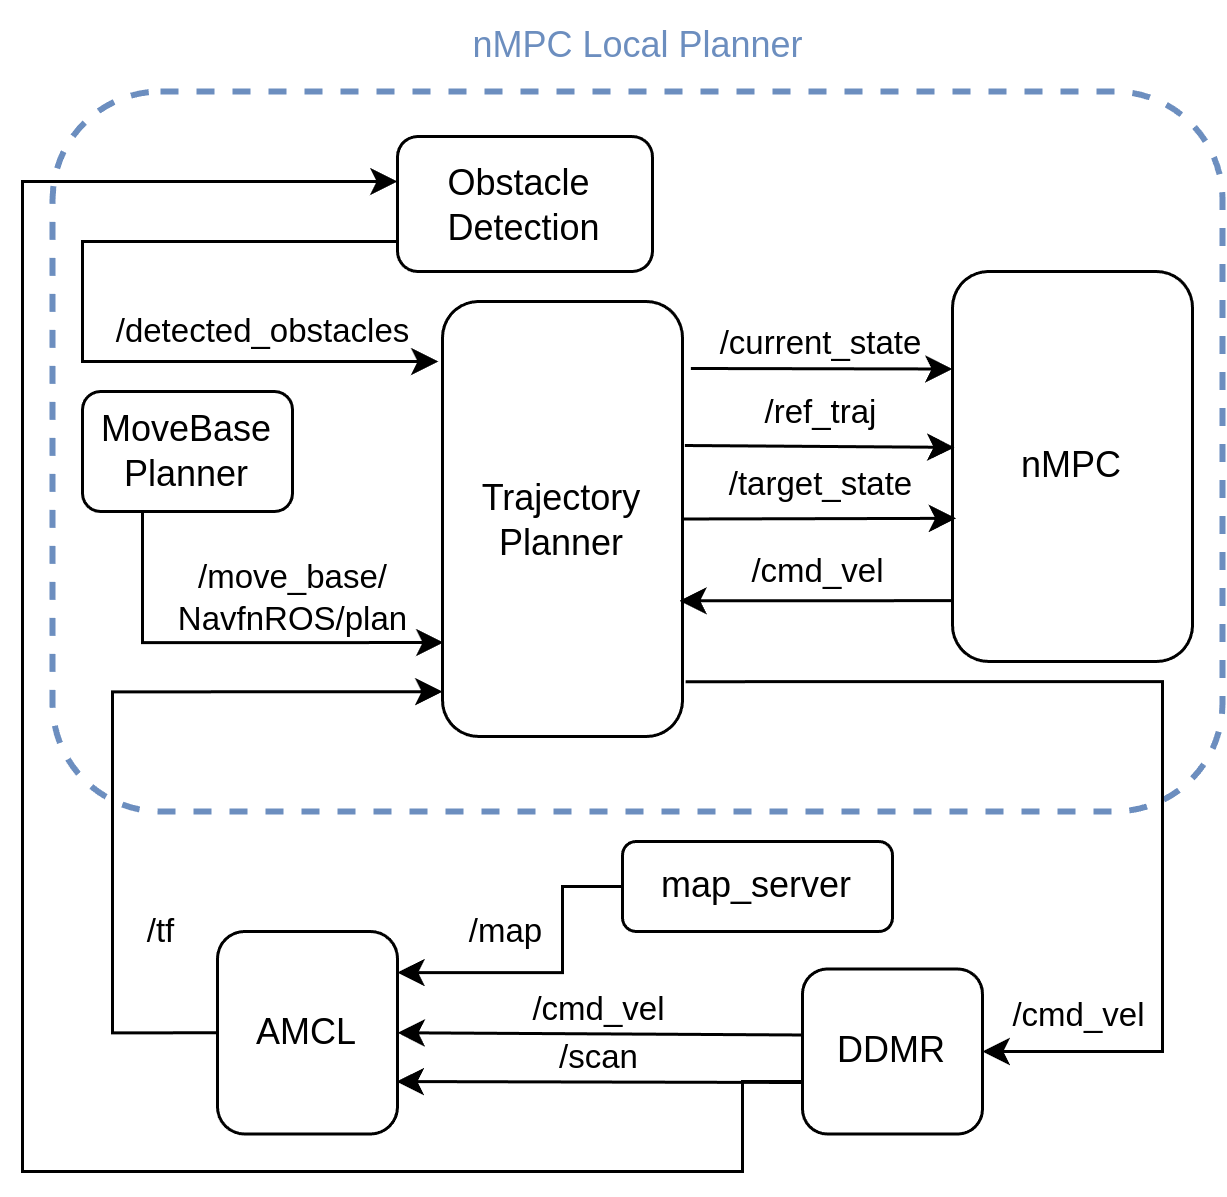
\includegraphics[width=1\columnwidth]{images/nMPC_Local_Planner_Diagram_2.png}
    \caption{nMPC-Local-Planner Block Diagram }
    \label{fig:nMPC_Local_Planner_Diagram_2}
\end{figure}


\subsection{Nonlinear Model Predictive Controller}

The nMPC is responsible for planning a path based on the current pose, the target pose, and the reference trajectory, using an optimizer that not only satisfies the kinematics of a differential drive mobile robot (DDMR) but also avoids obstacles and respects limitations on control inputs and States. Figure \ref{fig:nMPC_Blockdiagram_2} illustrates the components of an nMPC \cite{falcone2007predictive}.

\begin{figure}[!h]
    \centering
    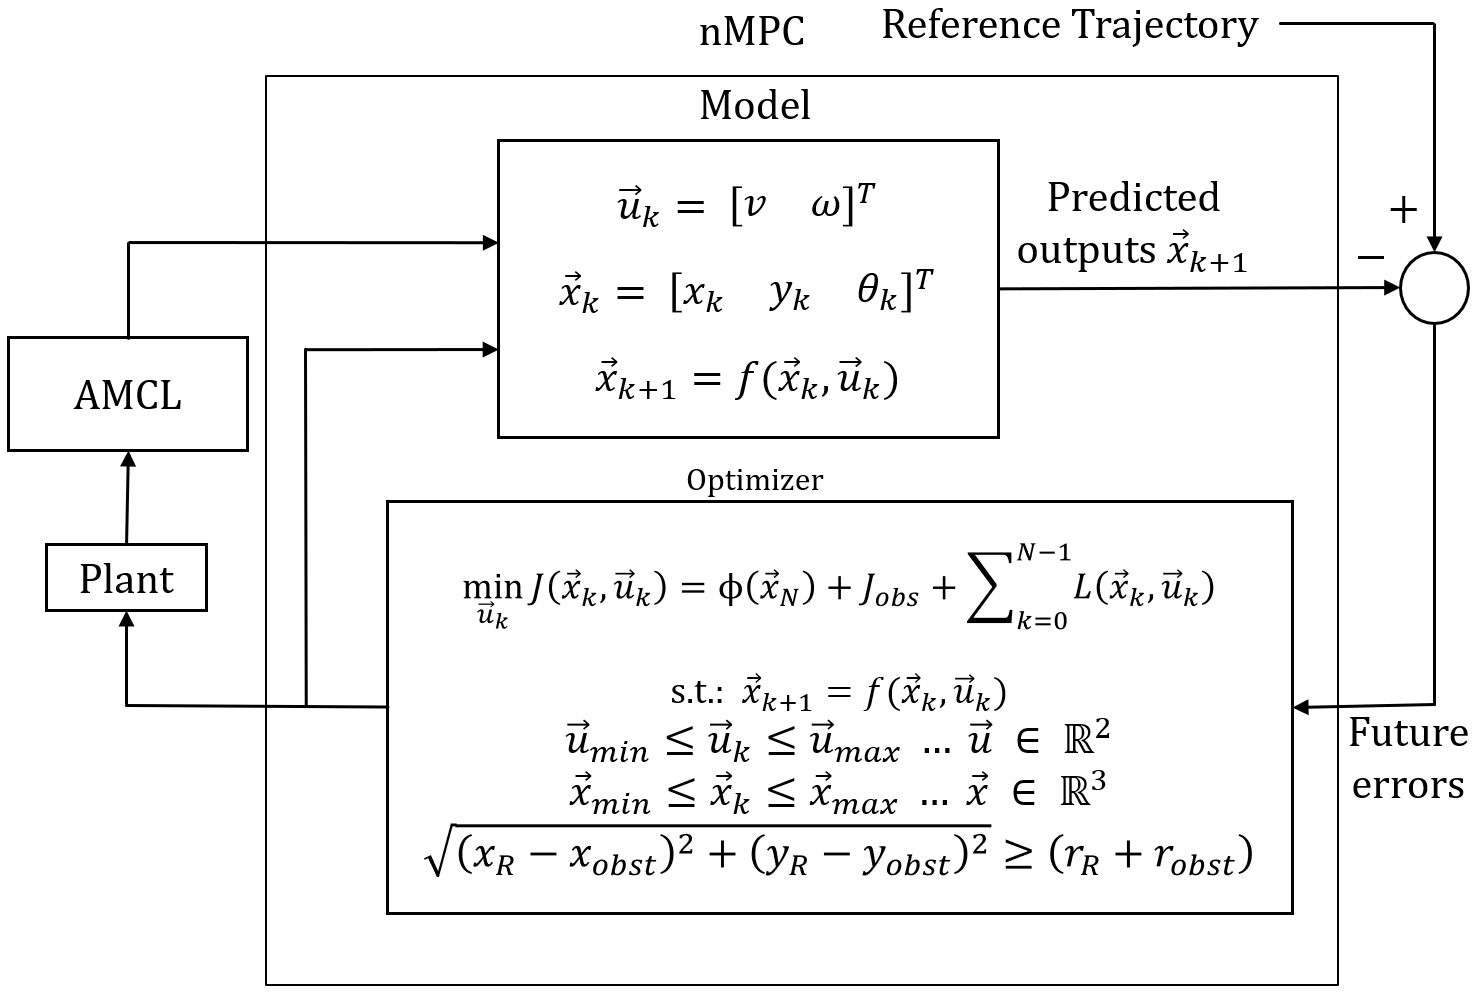
\includegraphics[width=1\columnwidth]{images/nMPC_Blockdiagram_2.png}
    \caption{Detailed Blockdiagram of nMPC (modified from \cite{Effects_of_roll_dynamics_for_car_stability_control_by_laguerre_functions})}
    \label{fig:nMPC_Blockdiagram_2}
\end{figure}

First, the Optimal Control Problem (OCP) must be converted into a Nonlinear Programming Problem (NLP) using the multiple shooting discretization method. Unlike single shooting, where only the control vector is optimized and the entire system is forward-simulated, multiple shooting introduces both the control vector and the state vector as optimization variables. This means that not only are the control inputs \( \mathbf{u} \) optimized, but the system states \( \mathbf{x} \) at each prediction step are also included in the optimization \cite{BOCK19841603}. 

The cost function (see Eq. \ref{eq:L_function}) is not merely a summation over all time steps, but instead, each segment's dynamics must adhere to the system's model equations, expressed as equality constraints (see Fig. \ref{fig:nMPC_Blockdiagram_2}). This enforces that the model dynamics are satisfied over the entire prediction horizon, and discrepancies between predicted and simulated states are minimized, improving both stability and accuracy \cite{DIEHL2002577}.

Moreover, this approach significantly enhances the computational time efficiency. By breaking the problem into smaller segments, the optimization solver can converge faster and more reliably, especially in the presence of complex nonlinear dynamics or large prediction horizons. The ability to treat state and control variables as separate optimization entities helps in avoiding divergence \cite{BOCK19841603}.

The goal is to minimize the cost function (see Eq. \ref{eq:L_function}), which consists of the States and control actions for all predictions \cite{rawlings2009model}.

\begin{equation}
\label{eq:L_function}
\begin{aligned}
\min_{\vec{u}_k} J(\vec{x}_k, \vec{u}_k) = J_{\text{obs}} + \phi(\vec{x}_N) 
+ &\\ \sum_{k}^{k+N-1}
(\vec{x}_{R,k} - \vec{x}_{\text{ref},k})^T Q (\vec{x}_{R,k} - \vec{x}_{\text{ref},k})&+ \vec{u}_k^T R \vec{u}_k
\end{aligned}
\end{equation}

The cost function \(J\) consists of three main components:
\begin{itemize}
    \item \(\phi(\vec{x}_N)\) represents the terminal cost, ensuring the final State \(\vec{x}_N\) is close to the target State, as defined in Equation \ref{eq:phi_definition} \cite{rawlings2009model}.
    \begin{equation}
    \label{eq:phi_definition}
    \phi(\vec{x}(N)) = \frac{1}{2} \vec{x}_N^T S \vec{x}_N
    \end{equation}

    \item \(J_{\text{obs}}\) is a penalty term that increases the cost if the robot comes close to an obstacle, calculated according to Equation \ref{eq:J_obs} \cite{frasch2013parallel}.
\end{itemize}

\begin{equation}
\label{eq:J_obs}
J_{\text{obs}} = \sum_{k=0}^{N} \sum_{i=1}^{n_{\text{obs}}} \frac{w_{\text{pen}}}{\sqrt{(x_k - x_{\text{obs},i})^2 + (y_k - y_{\text{obs},i})^2} + \epsilon}
\end{equation}

where \(x_{\text{obs},i}\) and \(y_{\text{obs},i}\) represent the coordinates of the \(i\)-th obstacle, and \(\epsilon\) is a small value to avoid singularities. 
The State vector \(\mathbf{x}\) and control vector \(\mathbf{u}\) are defined in Equations \ref{eq:State_vector} and \ref{eq:control_vector}, respectively \cite{liniger2015nonlinear}.

\begin{equation}\label{eq:State_vector}
    \mathbf{x}_k = \begin{bmatrix} x_k & y_k & \theta_k \end{bmatrix}^T
\end{equation}

\begin{equation}\label{eq:control_vector}
    u_k = \begin{bmatrix}
    v_k & \omega_k
\end{bmatrix}^T
\end{equation}

These vectors describe the position, orientation, and control inputs of the robot at each time step \(k\). The evolution of the State is constrained to follow the robot's kinematics, as enforced by Equation \ref{eq:discrete_dynamics} \cite{liniger2015nonlinear}.

\begin{align}
\vec{x}(k+1) &= f(\vec{x}(k), \vec{u}(k)) \label{eq:discrete_dynamics} \\
\vec{x}(0) &= \vec{x}_0
\end{align}

For a differential drive mobile robot, the discrete State-space dynamics are modeled as shown in Equation \ref{eq:discrete_State_space_equation_DDMR} \cite{thrun2005probabilistic}.

\begin{equation} \label{eq:discrete_State_space_equation_DDMR}
\begin{bmatrix}
    x_{k+1} \\
    y_{k+1} \\
    \theta_{k+1}
\end{bmatrix}
=
\begin{bmatrix}
    x_k \\
    y_k \\
    \theta_k
\end{bmatrix}
+ \Delta T
\begin{bmatrix}
    \cos(\theta_k) & 0 \\
    \sin(\theta_k) & 0 \\
    0 & 1
\end{bmatrix}
u_k
\end{equation}

To ensure safe navigation, the control inputs are constrained between the bounds specified in Equation \ref{eq:u_constraints}.

\begin{equation}
\label{eq:u_constraints}
\vec{u}_{\text{min}} \leq \vec{u}_k \leq \vec{u}_{\text{max}}, \quad \forall k
\end{equation}

In addition, a collision avoidance constraint, as shown in Equation \ref{eq:collision_condition}, ensures that the robot maintains a safe distance from obstacles.

\begin{equation}
\label{eq:collision_condition}
-\sqrt{(x_R - x_{\text{obst}})^2 + (y_R - y_{\text{obst}})^2} + (r_R + r_{\text{obst}}) \leq 0
\end{equation}

This inequality guarantees that the robot's distance from any obstacle is greater than or equal to the sum of their radii, preventing collisions \cite{frasch2013parallel}.

The control strategy computes the optimal sequence of control inputs \(\mathbf{u}_k\) by solving the NLP at each time step, taking into account the robot's current and predicted future States. The horizon \(N\) and the sampling time \(\Delta T\) influence how far ahead the controller predicts and adjusts the control actions.
By combining trajectory planning, obstacle avoidance, and constrained optimization, nMPC provides an integrated approach for navigating in dynamic environments.


\subsection{Trajectory Planner}

The trajectory planner processes the global path provided by the global planner and transforms it into a local path that adheres to the predictive horizon \( N \) of the nMPC and the predicted distance \( d_{\text{pred}} \). By default, the global planner in ROS assigns the same orientation to all waypoints, which is suboptimal for precise trajectory tracking. To address this, the orientation of each waypoint based on the direction to the next point along the path has been implemented. This results in waypoints that are aligned with the trajectory, improving navigation accuracy.

Once the waypoints are oriented correctly, they are passed to the trajectory interpolation algorithm. This algorithm ensures that the number of waypoints matches the number of nMPC predictions. Based on the robot's maximum linear velocity \( v_{\text{max}} \), the algorithm calculates the appropriate time stamps for the interpolated local path. This guarantees that the nMPC maintains the correct prediction length. Additionally, the time constant is multiplied by a scaling factor \( \alpha \) to generate a feedforward effect, ensuring that the reference waypoints are always ahead of the robot's current State, guiding the robot to follow the trajectory effectively. This technique also allows for subtle manipulation of speed along the trajectory.

A plot illustrating this interpolation process is provided in Figure \ref{fig:nMPC_Interpolation_Plot}. In the example, three waypoints are given, and the algorithm linearly interpolates 10 points for 10 predictions.


\begin{algorithm}
\caption{Trajectory Interpolation. Variables: $P = \{(x_i, y_i, \text{yaw}_i)\}$, $d_{\text{pred}}$, $N$, $v_{\text{max}}$, $\alpha$}
\begin{algorithmic}[1]
\State Compute cumulative distance between points:
\[
D_i = \sum \sqrt{(x_{i+1} - x_i)^2 + (y_{i+1} - y_i)^2}
\]
\State Retain points where $D_i \leq d_{\text{pred}}$
\State Compute interpolated distance per point:
\[
d_{\text{point}} = \frac{d_{\text{pred}}}{N}
\]
\State Compute time step based on maximum velocity:
\[
T = \frac{d_{\text{point}}}{v_{\text{max}}}
\]
\State Adjust time step with scaling factor:
\[
T = T \cdot \alpha
\]
\State Interpolate $x$, $y$, and $\text{yaw}$ to get $N$ prediction points
\State \textbf{return} $P_{\text{new}}$, $T$
\end{algorithmic}
\end{algorithm}


This interpolation algorithm takes the reference global path and generates \( N \) evenly spaced points along the trajectory. The associated time step \( T \) ensures smooth and continuous control of the robot’s motion, with feedforward control helping to keep the reference trajectory ahead of the robot’s actual State. This approach is analogous to the method used in the TEB Local Planner \cite{ROSMANN2017142}.

\begin{figure}[!h]
    \centering
    \includegraphics[width=1\columnwidth]{images/Interpolated_Trajectories.png}
    \caption{Interpolation process: Given 3 initial waypoints, 10 linearly interpolated waypoints are generated for 10 nMPC predictions.}
    \label{fig:nMPC_Interpolation_Plot}
\end{figure}


\subsection{Obstacle Detection}

Unlike DWA and TEB, the obstacle detection algorithm does not subscribe to the local costmap but instead directly processes laser scan data. The laser scan data, once received, are initially filtered based on a search cone, defined by the search radius and search angle, as illustraded in Algorithm \ref{alg:Obstacle_Detection_Algorithm}. This filtering step helps to exclude obstacles that are behind the robot and no longer relevant. The nMPC is currently designed to operate only with positive linear velocities, meaning the robot is expected to move forward. If backward motion were required, the search angle would need to be adjusted by 180°.

After filtering, the scan data are transformed into 2D coordinates to create a LiDAR image. The LiDAR image is then smoothed using Gaussian blur, which helps reduce noise and makes obstacle detection more robust. The smoothing process is critical for ensuring the corner detection algorithm functions effectively, as it eliminates irregularities and helps detect more consistent object edges. The Shi-Tomasi corner detection algorithm is applied to identify obstacles, by detecting corners \cite{GoodFeaturesToTrack}. Initially intended for corner detection, the algorithm can also detect walls or flat surfaces depending on the quality level, likely due to the inherent noise in the sensor data. By sending only the most relevant obstacles to the nMPC, the computational load is minimized, allowing for real-time decision-making.


Once corners are detected, they are sorted by their distance from the robot. The detected positions are then transformed to the robot's coordinate frame. Finally, only the maximum number of obstacles that the nMPC can process are considered, with any additional obstacles being discarded, ensuring that the closest obstacles are considered by the planner.

\begin{algorithm}
\caption{Shi-Thomas Obstacle Detection}
\label{alg:Obstacle_Detection_Algorithm}
\begin{algorithmic}[1]
\State Filter laser scan data $(r_i, \theta_i)$ using:
\[
r_i < r_{\text{search}} \quad \text{and} \quad \left( -\frac{\theta_{\text{search}}}{2} \leq \theta_i \leq \frac{\theta_{\text{search}}}{2} \right)
\]
\State Convert filtered data to 2D coordinates:
\[
x_i = r_i \cos(\theta_i), \quad y_i = r_i \sin(\theta_i)
\]
\State Create a LiDAR image for obstacle detection:
\begin{align*}
x_{\text{img}} &= \left( \frac{x_i}{r_{\text{max}}} \times I_{\text{size}} \right) + \frac{I_{\text{size}}}{2}, \\
y_{\text{img}} &= \left( \frac{y_i}{r_{\text{max}}} \times I_{\text{size}} \right) + \frac{I_{\text{size}}}{2}
\end{align*}
\State Apply Gaussian blur to smooth the image:
\[
I_{\text{blur}}(x, y) = \frac{1}{2\pi \sigma^2} \exp\left(-\frac{x^2 + y^2}{2\sigma^2}\right) \otimes I_{\text{img}}(x, y)
\]
\State Detect corners using the Shi-Tomasi corner detection algorithm:
\[
\{(x_{\text{corner}}, y_{\text{corner}})\} = \text{Shi-Tomasi}(I_{\text{blur}})
\]
\State Sort detected corners by distance from the robot:
\[
d_i = \sqrt{x_{\text{corner}}^2 + y_{\text{corner}}^2}
\]
\State Transform detected corners into the robot’s frame of reference:
\[
x_{\text{trans}} = x_{\text{robot}} + (x_{\text{corner}} \cos(\text{yaw}) - y_{\text{corner}} \sin(\text{yaw}))
\]
\[
y_{\text{trans}} = y_{\text{robot}} + (x_{\text{corner}} \sin(\text{yaw}) + y_{\text{corner}} \cos(\text{yaw}))
\]
\State Select $N_{\text{max}}$ closest points
\State \textbf{return} $(x_{\text{trans}}, y_{\text{trans}}, r_{\text{corner}})$ to nMPC
\end{algorithmic}
\end{algorithm}

A visual representation of the obstacle detection algorithm is shown in Figure \ref{fig:Obstacle_Detection}, illustrating how the laser scan data are filtered, converted, and processed to detect obstacles before passing the data to the nMPC.

\begin{figure}[!h]
    \centering
    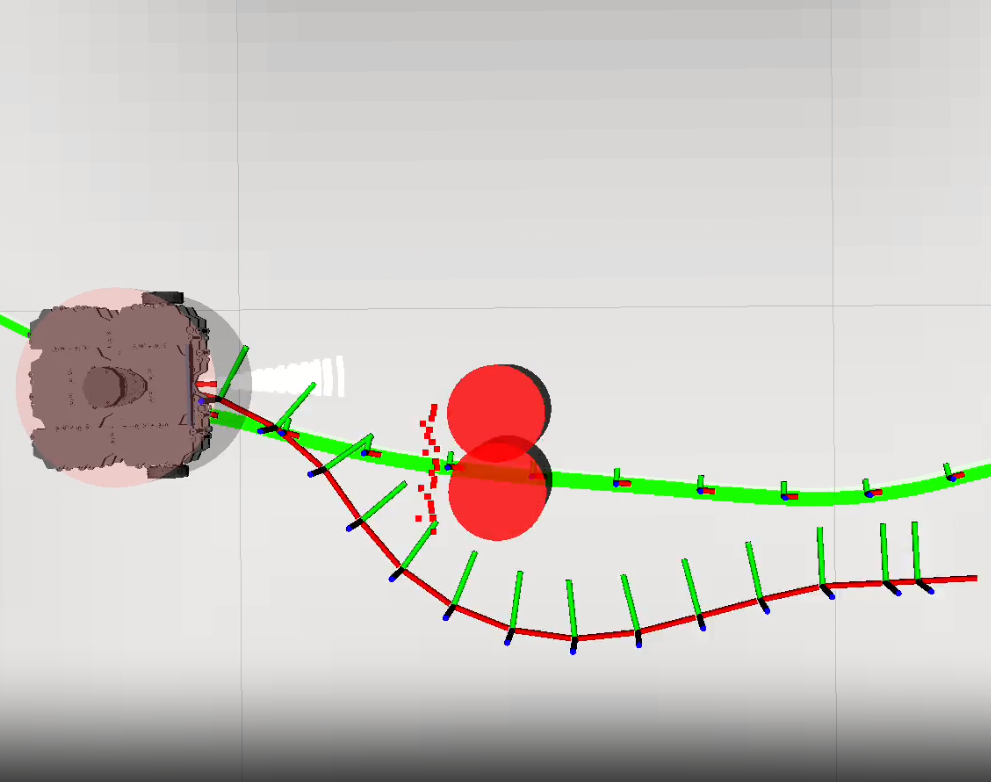
\includegraphics[width=1\columnwidth]{images/obstacle_detection_2.png}
    \caption{Obstacle Detection Algorithm in which the DDMR detects a cube with the scan measurement and representing it as two circles}
    \label{fig:Obstacle_Detection}
\end{figure}

The integration of the obstacle detection algorithm with the trajectory interpolation ensures that the nMPC can safely navigate through the environment while considering both the robot’s kinematics and the presence of dynamic obstacles.


%%%%%%%%%%%%%%%%%%%%%%%%%%%%%%%%%%%%%%%%%%%%%%%%%%%%%%%%%%%%%%%%%%
\section{Implementation Detail}
\subsection{CasADi}

CasADi was chosen for this work due to its robust framework, which integrates with IPOPT to perform nonlinear optimizations. For the implementation of the nMPC, it was necessary to predefine the optimization problem in CasADi. This involved defining all the required matrices for the State vector, control vector, optimization variables, and weighting matrices \( Q \), \( R \) and \( S \), as well as the cost function.

When the optimization problem is called, all necessary parameters are passed, including the current State, the reference trajectory, obstacles (represented as \( n \)-times \((x, y, \text{radius})\)), and the computed time constant \( T \). The parameter settings for the optimization solver were configured as follows:

\begin{lstlisting}
opts = {'ipopt.max_iter': 2000,
        'ipopt.print_level': 0,
        'print_time': 0,
        'ipopt.acceptable_tol': 1e-8,
        'ipopt.acceptable_obj_change_tol': 1e-6}
\end{lstlisting}


\subsection{Software Setup}

The system was implemented in ROS1 due to its existing Navigation Stack, which includes State-of-the-art local planners such as DWA and TEB. ROS1 provides a simple and efficient way to integrate, test, and validate the nMPC alongside these well-established planners. Additionally, ROS1 offers an open-source platform, making it possible for the community to further test and develop the system. Additionally, this work was containerized using Docker to ensure a consistent development environment, simplifying deployment and facilitating collaboration.

% \subsection{Evaluation Metrics}

% The experiments were conducted using three key metrics:

% \begin{itemize}
%     \item Cross Tracking Error: The deviation of the robot's path from the first reference trajectory.
%     \item Arrival Time: The time taken for the robot to reach its target waypoint.
%     \item Computation Time: The average time required for the local planner to compute the control inputs.
% \end{itemize}

% \subsubsection{Experiment 1: Dynamic Obstacle Avoidance}

% In the first experiment, the robot is tasked with navigating to a waypoint on the map. During this task, a dynamic obstacle moves in a circular pattern within the Gazebo simulation. The obstacle is detected only by the LiDAR sensors and the local costmap, but is not accounted for in the global plan. The update frequency of the system is reduced to 1 Hz, making the local planner responsible for most of the planning decisions, instead of the global planner. The performance of the three local planners—nMPC, DWA, and TEB—was measured based on the predefined metrics, with particular attention given to observing whether any of the planners collided with the rotating obstacle.

% \subsubsection{Experiment 2: Narrow Passage with Static Obstacle}

% In the second experiment, the robot must pass through a narrow corridor. However, the passage is partially blocked by a static obstacle, which is not present in the pre-mapped environment. Consequently, the global planner generates a plan that passes through the "invisible" obstacle, requiring the local planner to detect and avoid it. The performance of the local planners was again evaluated using the same metrics.

% \subsubsection{Ablation Experiment: Disabled LiDAR Scans}

% In the ablation experiment, each local planner is required to navigate to a target point. The direct path is obstructed by a mapped object, and the LiDAR scan data are disabled to test the robustness of the planners without the aid of real-time obstacle detection. This scenario was designed to assess how well the planners perform when relying solely on pre-mapped data.

\subsection{Hardware}

The experiments were conducted on a system equipped with an AMD Ryzen 5 7600X 6-Core Processor running at a maximum clock speed of 5.45 GHz. The system has 12 logical CPUs (2 threads per core) and 30 GB of RAM, with no swap space configured.

The experiments ran inside a Docker container, which utilized up to 4.808 GB of RAM (approximately 15.78 \% of the available memory) and had a peak CPU usage of 855.20 \%, indicating multi-core processing. The container handled a maximum of 393 processes during the experiments.

%%%%%%%%%%%%%%%%%%%%%%%%%%%%%%%%%%%%%%%%%%%%%%%%%%%%%%%%%%%%%%%%%%
\section{Discussion and Results}
In this section, the results are presented in detail and evaluated on the basis of the previously defined metrics, such as cross-tracking error, arrival time and calculation time. It analyses how well the developed nMPC Local Planner performed in comparison to other methods such as DWA and TEB. In particular, the extent to which the soft and hard constraints used contributed to obstacle avoidance and the role that parameters such as prediction length and obstacle detection played in performance in dynamic environments are discussed.

\subsection{Evaluation Metrics}

The experiments were conducted using three key metrics:

\begin{itemize}
    % CTE
    \item Cross Tracking Error: The CTE measures the accuracy of path tracking by calculating the minimum distance from the robot's path to the reference trajectory. This metric helps evaluate how well the robot follows the desired path \cite{gonzalez2015review}.
    
    \begin{multline}
    CTE = \frac{1}{N} \sum_{i=1}^{N} \min \Bigg( \sqrt{(x_{\text{robot}, i} - x_{\text{global}, j})^2} \\
    + \sqrt{(y_{\text{robot}, i} - y_{\text{global}, j})^2} \Bigg)
    \label{eq:CTE}
    \end{multline}
    
    where \( N \) is the total number of points along the path. \( (x_i, y_i) \) represents the coordinates of the actual position of the robot at point \(i\), and \( (x_{\text{ref},i}, y_{\text{ref},i}) \) are the coordinates of the reference path. The term inside the square root is the Euclidean distance between the actual position and the reference path at each point, and the minimum selects the closest point on the path.

    % Arrival Time
    \item Arrival Time: This metric measures the time taken for the robot to reach its target waypoint. It is crucial for evaluating the efficiency of local planners, especially in dynamic environments where timely responses are important \cite{werling2012optimal}.
    
    % Computation Time
    \item Computation Time: The average time required for the local planner to compute the control inputs is used to assess real-time performance (see Eq. \ref{eq:comp_time_correct}). This helps evaluate the planner's efficiency in generating control inputs quickly \cite{nielsen2020real}.
    
    \begin{equation}
    t_{\text{comp}} = \frac{1}{N-1} \sum_{i=1}^{N-1} (t_{i+1} - t_i)
    \label{eq:comp_time_correct}
    \end{equation}
    
    where \( N \) is the total number of `cmd\_vel` messages, \( t_i \) is the timestamp of the \( i \)-th message, and \( t_{i+1} - t_i \) represents the time difference between consecutive messages.
\end{itemize}

\subsubsection{Experiment 1: Dynamic Obstacle Avoidance}

In the first experiment, the robot is tasked with navigating to a waypoint on the map. During this task, a dynamic obstacle moves in a circular pattern within the Gazebo simulation. The obstacle is detected only by the LiDAR sensors and the local costmap, but is not accounted for in the global plan. The update frequency of the system is reduced to 1 Hz, making the local planner responsible for most of the planning decisions, instead of the global planner. The performance of the three local planners—nMPC, DWA, and TEB—was measured based on the predefined metrics, with particular attention given to observing whether any of the planners collided with the rotating obstacle.

\subsubsection{Experiment 2: Narrow Passage with Static Obstacle}

In the second experiment, the robot must pass through a narrow corridor. However, the passage is partially blocked by a static obstacle, which is not present in the pre-mapped environment. Consequently, the global planner generates a plan that passes through the "invisible" obstacle, requiring the local planner to detect and avoid it. The performance of the local planners was again evaluated using the same metrics.

\subsubsection{Ablation Experiment: Disabled LiDAR Scans}

In the ablation experiment, each local planner is required to navigate to a target point. The direct path is obstructed by a mapped object, and the LiDAR scan data are disabled to test the robustness of the planners without the aid of real-time obstacle detection. This scenario was designed to assess how well the planners perform when relying solely on pre-mapped data.


Each experiment is first presented with an XY plot showing the paths generated by the three local planners (nMPC, DWA, and TEB) alongside the initial global path. Following this, a bar chart is provided that compares the three metrics—cross tracking error, computation time, and arrival time—across all three planners. This structure is consistently applied across all three experiments.

\subsection{Experiment 1: Dynamic Obstacle Avoidance}

In the first experiment in Figure \ref{fig:nMPC_22_vs_DWA_12_vs_TEB_6_Path}, the TEB planner encountered significant challenges with the rotating obstacle. The TEB planner entered a deadlock situation, where the elastic band surrounding the robot's path became entangled with the rotating obstacle. This prevented the planner from finding a valid path, resulting in a collision with the obstacle. Once the planner switched to recovery mode, causing the robot to rotate in place and clear the local costmap, it was able to find a new path and reach the target. However, this process led to an extended arrival time of over 90 seconds, which can be seen in Figure \ref{fig:nMPC_22_vs_DWA_12_vs_TEB_6}, and the cross tracking error with respect to the global path was also considerable due to the repeated rotations caused by the rotating obstacle.

In contrast, both the nMPC and DWA planners successfully reached their targets in 40 and 39 seconds, respectively. The DWA planner achieved a slightly better cross tracking error than the nMPC (0.01 m difference), though the nMPC planner outperformed the DWA planner by being 2.3 times faster in computation time. While this difference is not captured in the plot, it was observed in the simulation that the DWA planner detected the obstacle only when it was directly in front of the robot, whereas the nMPC was able to predict and avoid the obstacle up to 2 meters in advance.

\begin{figure}[!h]
    \centering
    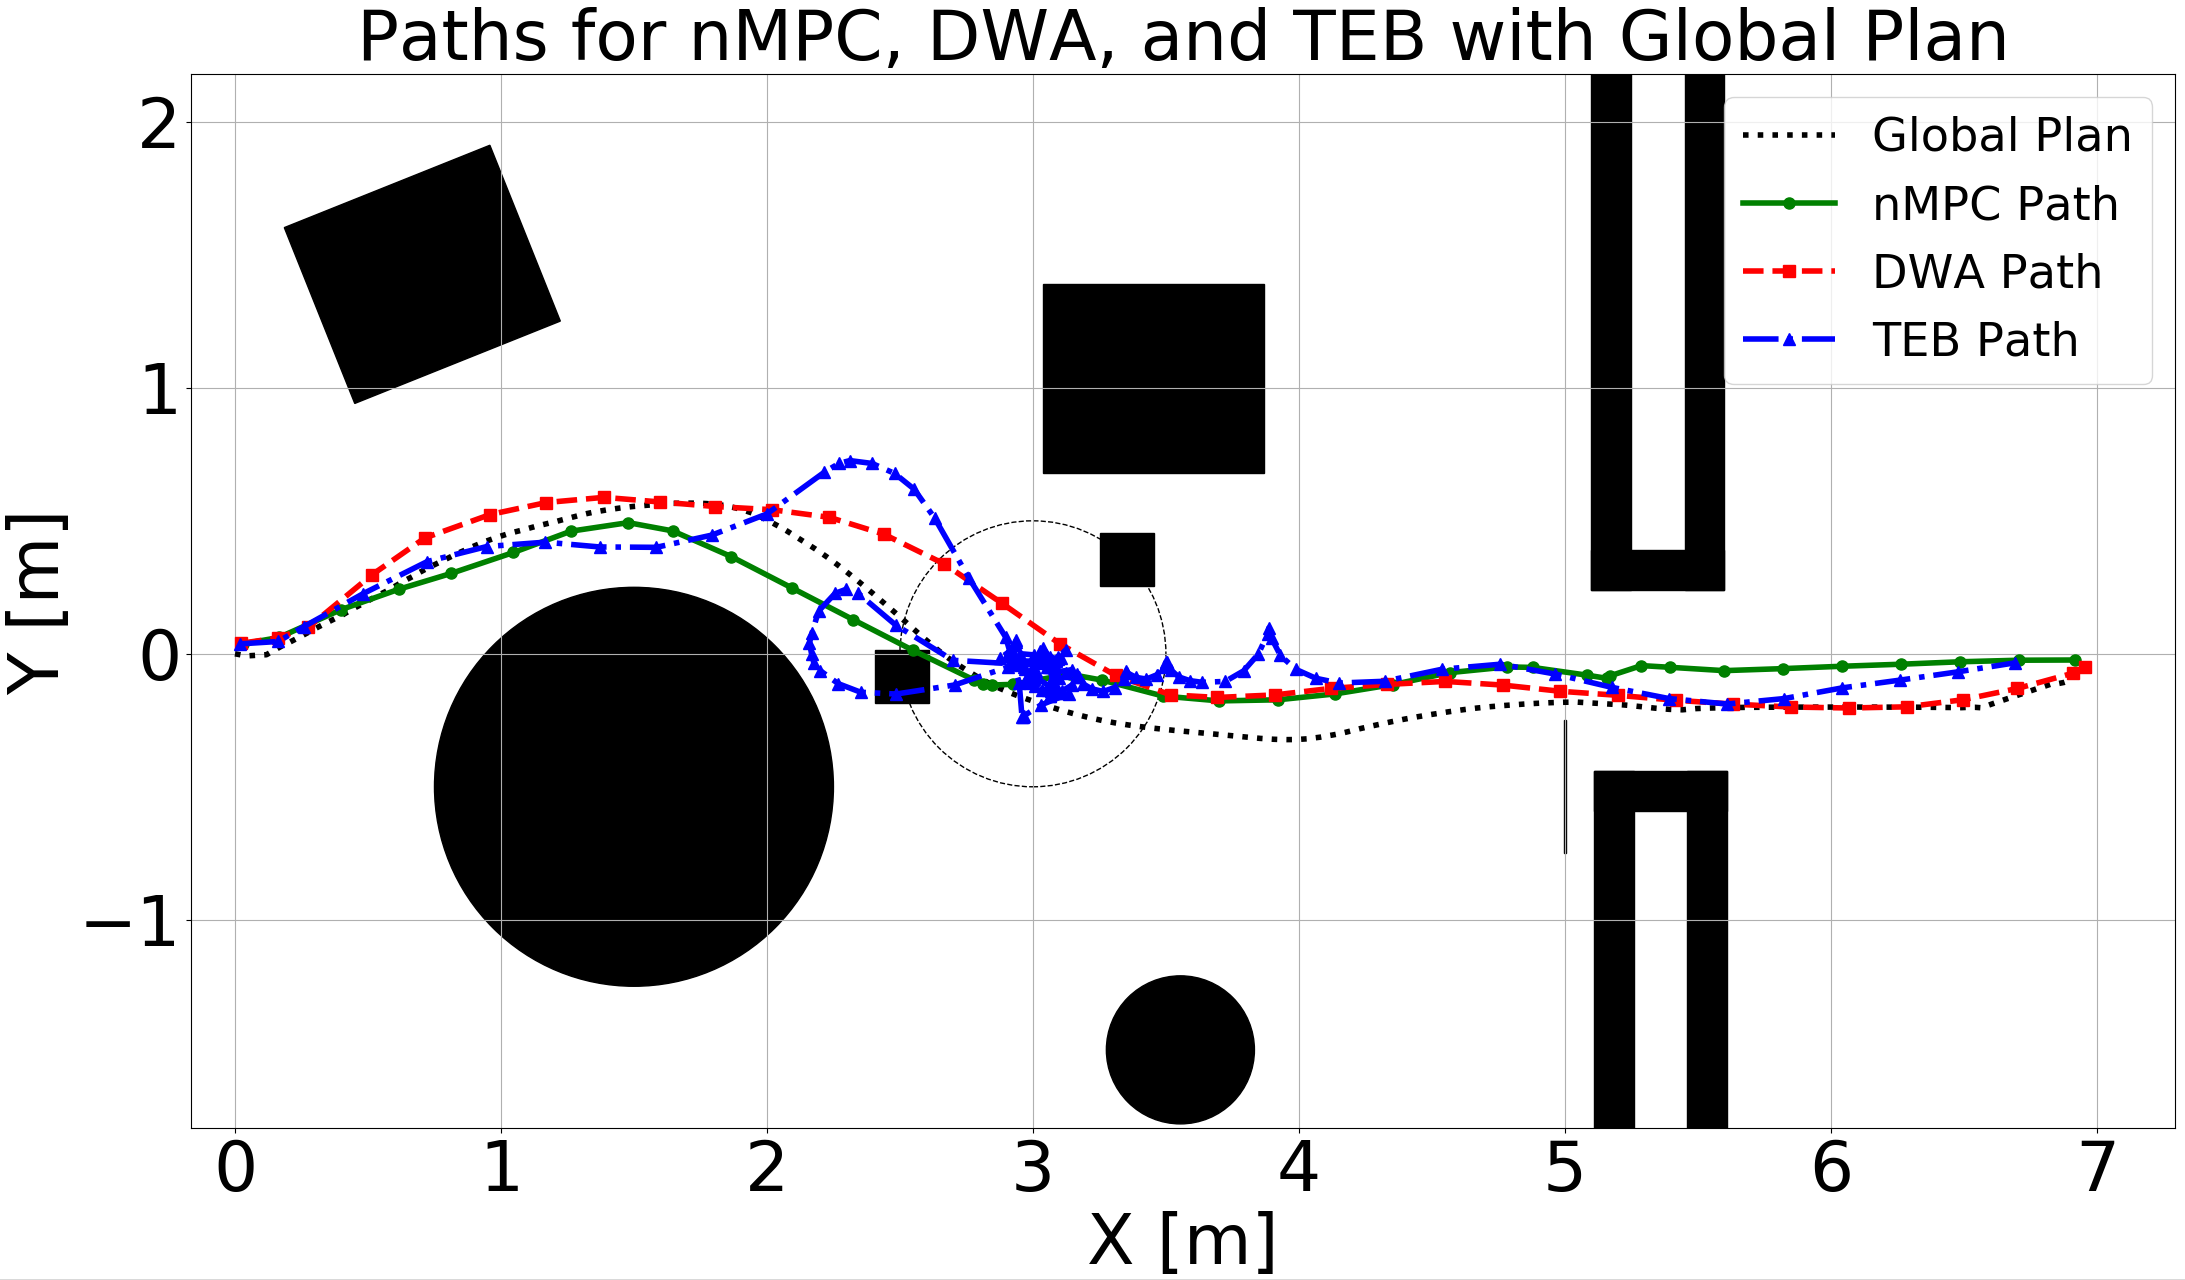
\includegraphics[width=1\columnwidth]{images/nMPC_22_vs_DWA_10_vs_TEB_8_Path.png}
    \caption{Comparison of paths for nMPC, DWA, and TEB in Experiment 1}
    \label{fig:nMPC_22_vs_DWA_12_vs_TEB_6_Path}
\end{figure}

\begin{figure}[!h]
    \centering
    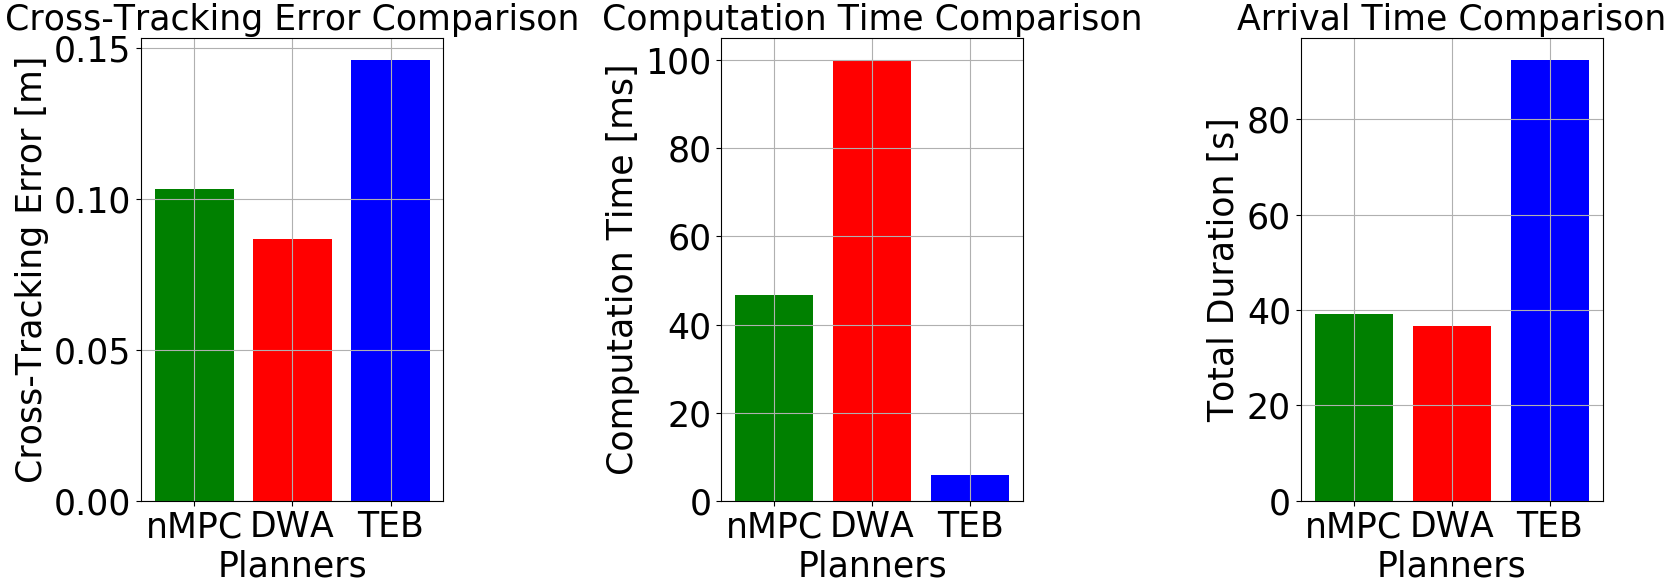
\includegraphics[width=1\columnwidth]{images/nMPC_22_vs_DWA_10_vs_TEB_8.png}
    \caption{Metrics comparison (cross tracking error, computation time, arrival time) for nMPC, DWA, and TEB in Experiment 1}
    \label{fig:nMPC_22_vs_DWA_12_vs_TEB_6}
\end{figure}

\subsection{Experiment 2: Narrow Passage with Static Obstacle}

In contrast to Experiment 1, the TEB planner was the fastest to reach the target in Experiment 2, completing the task in 15 seconds, followed closely by the nMPC planner at 18 seconds, which can be seen in Figure \ref{fig:nMPC_23_vs_DWA_12_vs_TEB_6}. The DWA planner, however, took significantly longer, with an arrival time of approximately 35 seconds. The delay in the DWA planner was attributed to its failure to account for the static obstacle blocking the passage. The global planner generated a path through the obstacle, and the DWA local planner was unable to compute a correction in time, resulting in repeated collisions with the wall.

Although the TEB planner reached the goal fastest, the nMPC planner achieved the lowest cross tracking error, demonstrating more precise path adherence. The TEB planner continued to show a consistent computation time of 5-10 ms as seen in Figure \ref{fig:nMPC_16_vs_DWA_12_vs_TEB_6}, \ref{fig:nMPC_22_vs_DWA_12_vs_TEB_6} and \ref{fig:nMPC_23_vs_DWA_12_vs_TEB_6}.

\begin{figure}[!h]
    \centering
    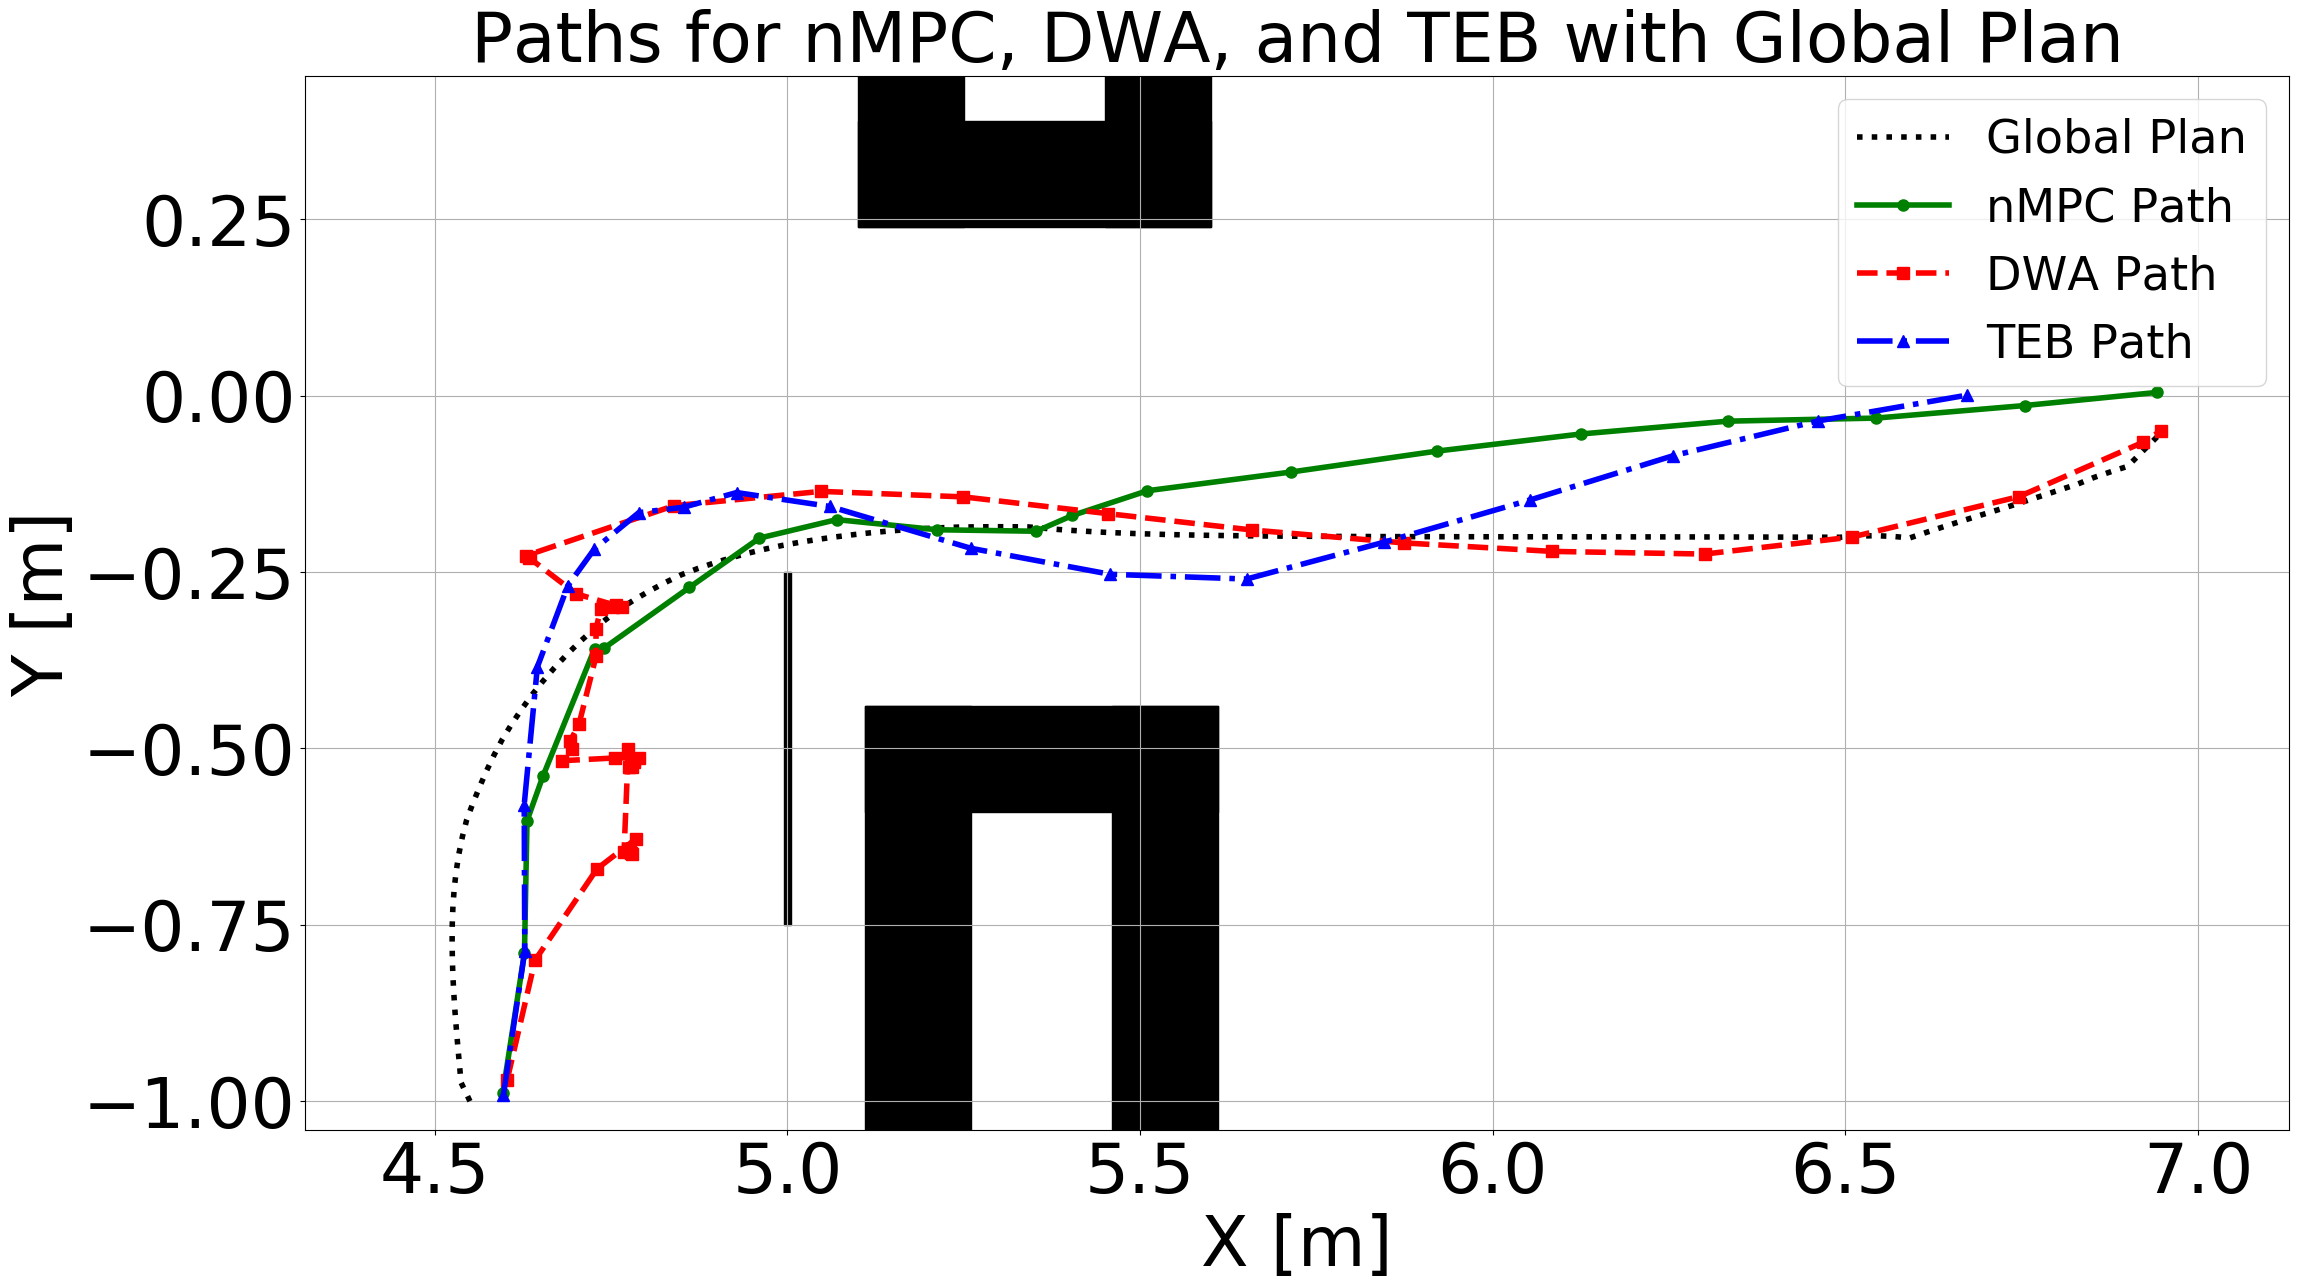
\includegraphics[width=1\columnwidth]{images/nMPC_23_vs_DWA_12_vs_TEB_9_Path.png}
    \caption{Comparison of paths for nMPC, DWA, and TEB in Experiment 2}
    \label{fig:nMPC_23_vs_DWA_12_vs_TEB_6_Path}
\end{figure}

\begin{figure}[!h]
    \centering
    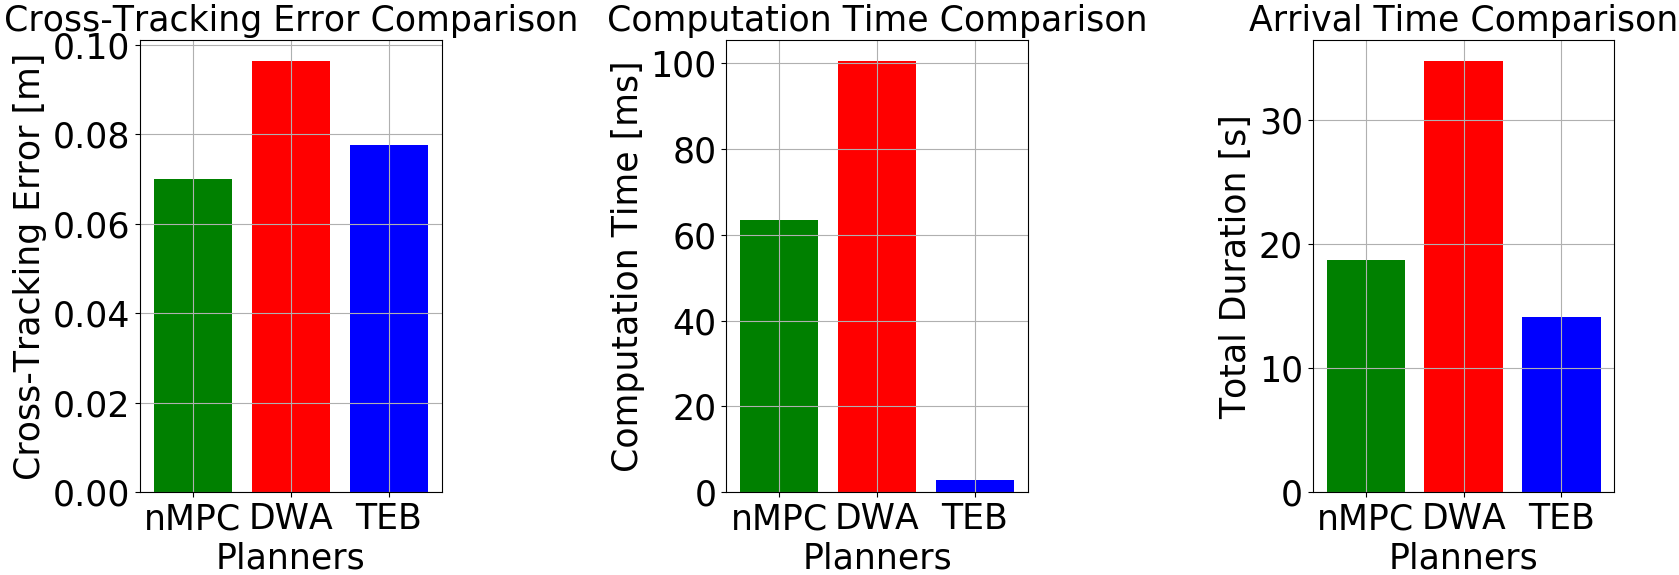
\includegraphics[width=1\columnwidth]{images/nMPC_23_vs_DWA_12_vs_TEB_9.png}
    \caption{Metrics comparison (cross tracking error, computation time, arrival time) for nMPC, DWA, and TEB in Experiment 2}
    \label{fig:nMPC_23_vs_DWA_12_vs_TEB_6}
\end{figure}

\subsection{Ablation Experiment: Lidar Scan Disabled}

In the final experiment, the nMPC planner failed to reach its target, colliding with an object due to the absence of scan data. A key limitation of the current nMPC implementation is that when the final goal falls within the prediction horizon, the controller switches from reference tracking to point stabilization to optimize performance. This behavior needs to be addressed to ensure the nMPC follows the entire trajectory, rather than stopping prematurely at the prediction horizon.

Despite reaching its goal, the TEB planner also collided with the object during this experiment. The DWA planner, in contrast, exhibited the best performance in terms of arrival time and cross tracking error when lidar scan data were disabled, demonstrating its robustness in situations where real-time obstacle detection is not available.

\begin{figure}[!h]
    \centering
    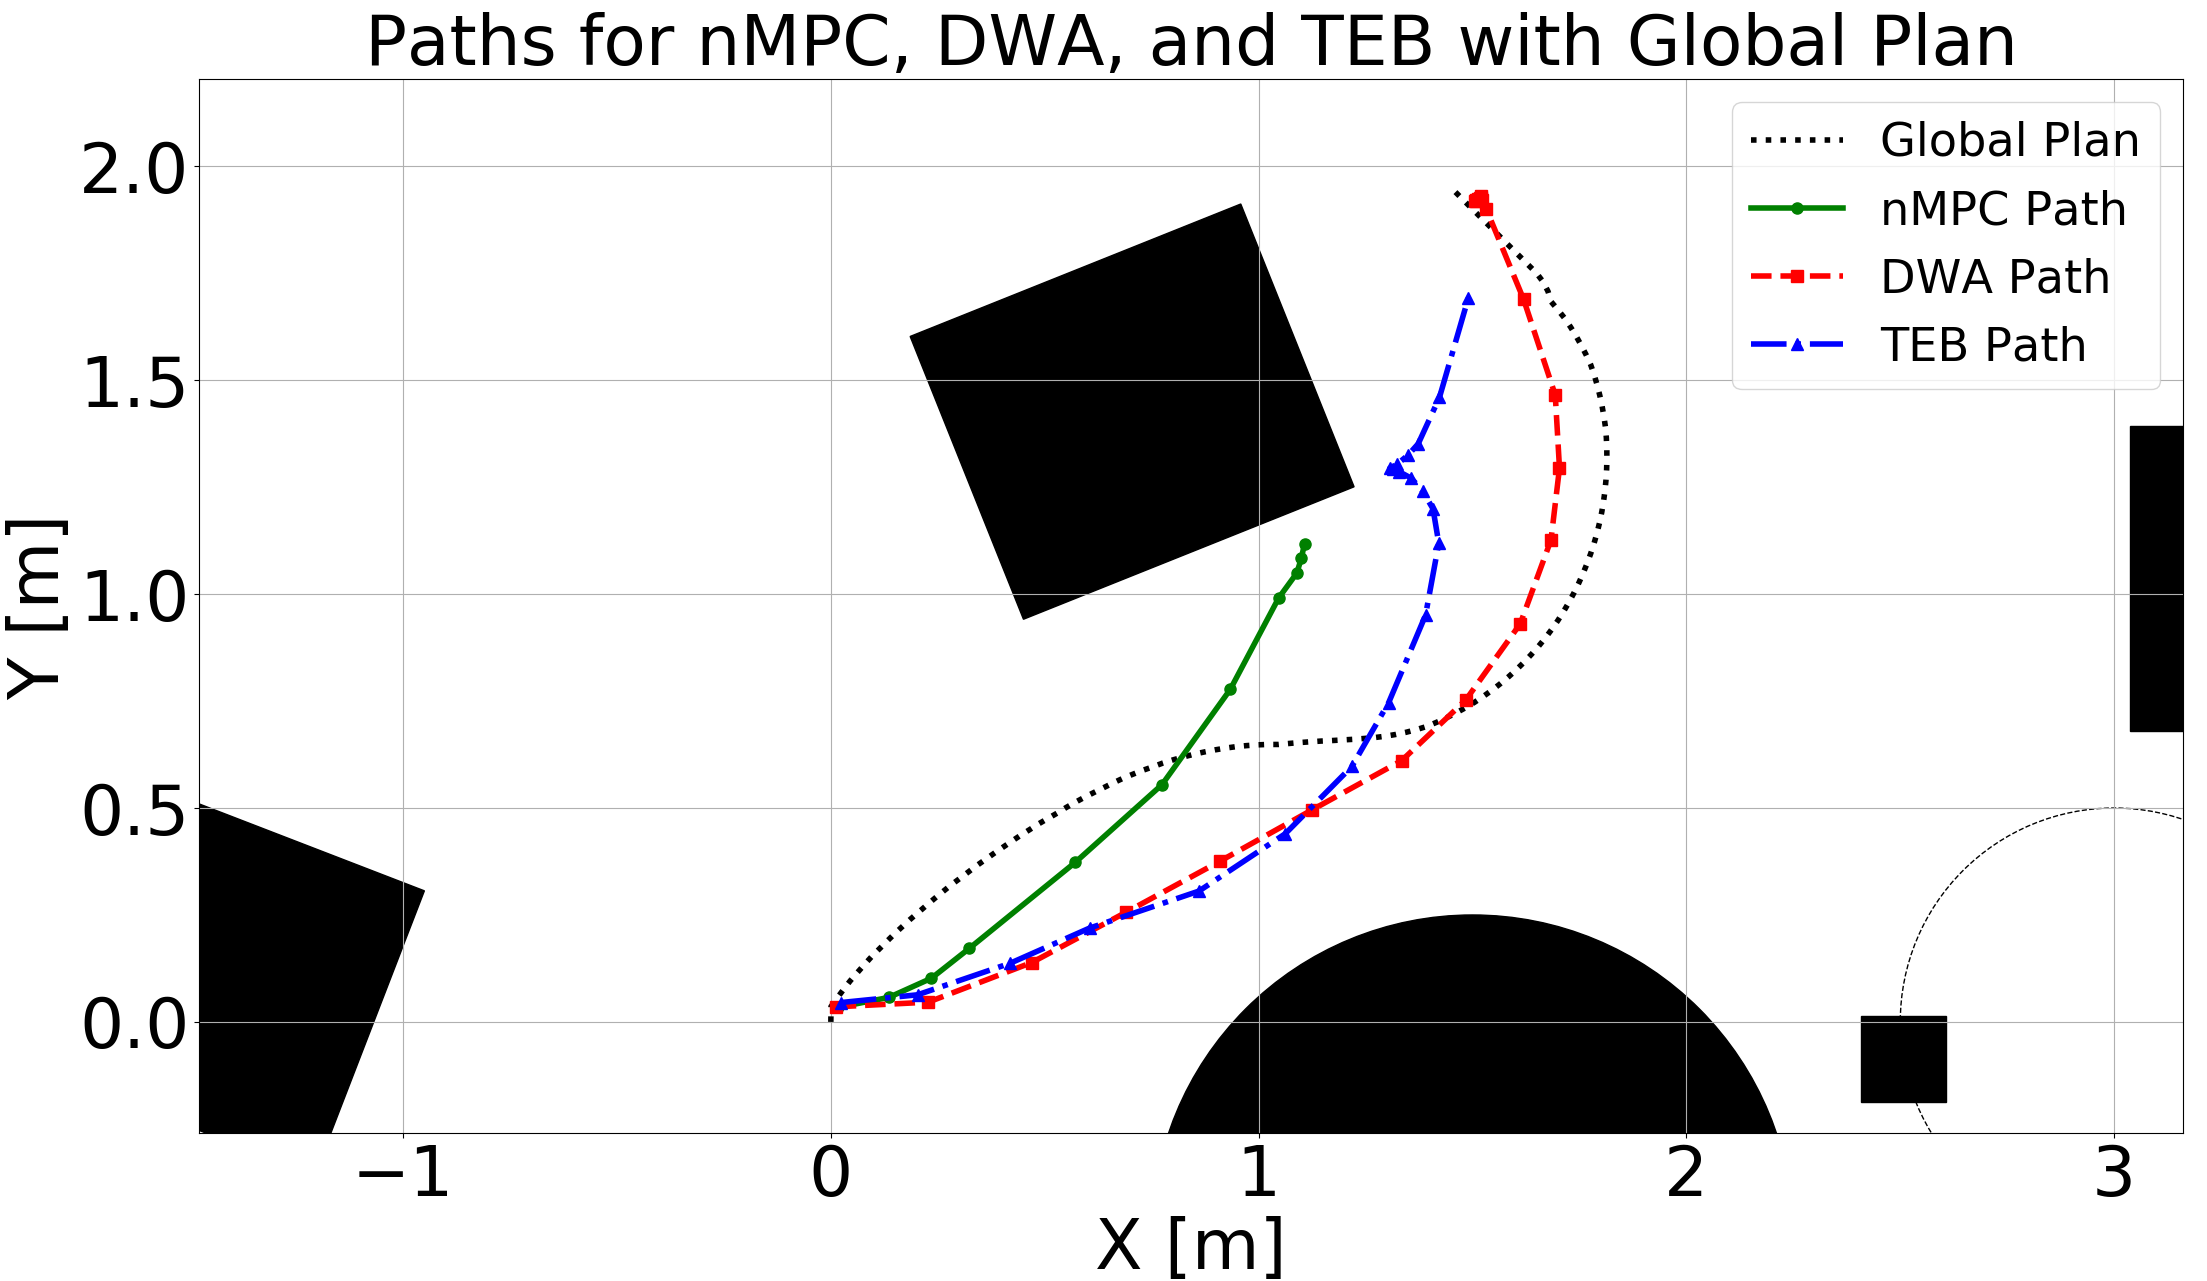
\includegraphics[width=1\columnwidth]{images/nMPC_18_vs_DWA_15_vs_TEB_10_Path.png}
    \caption{Comparison of paths for nMPC, DWA, and TEB in Ablation Experiment}
    \label{fig:nMPC_16_vs_DWA_12_vs_TEB_6_Path}
\end{figure}

\begin{figure}[!h]
    \centering
    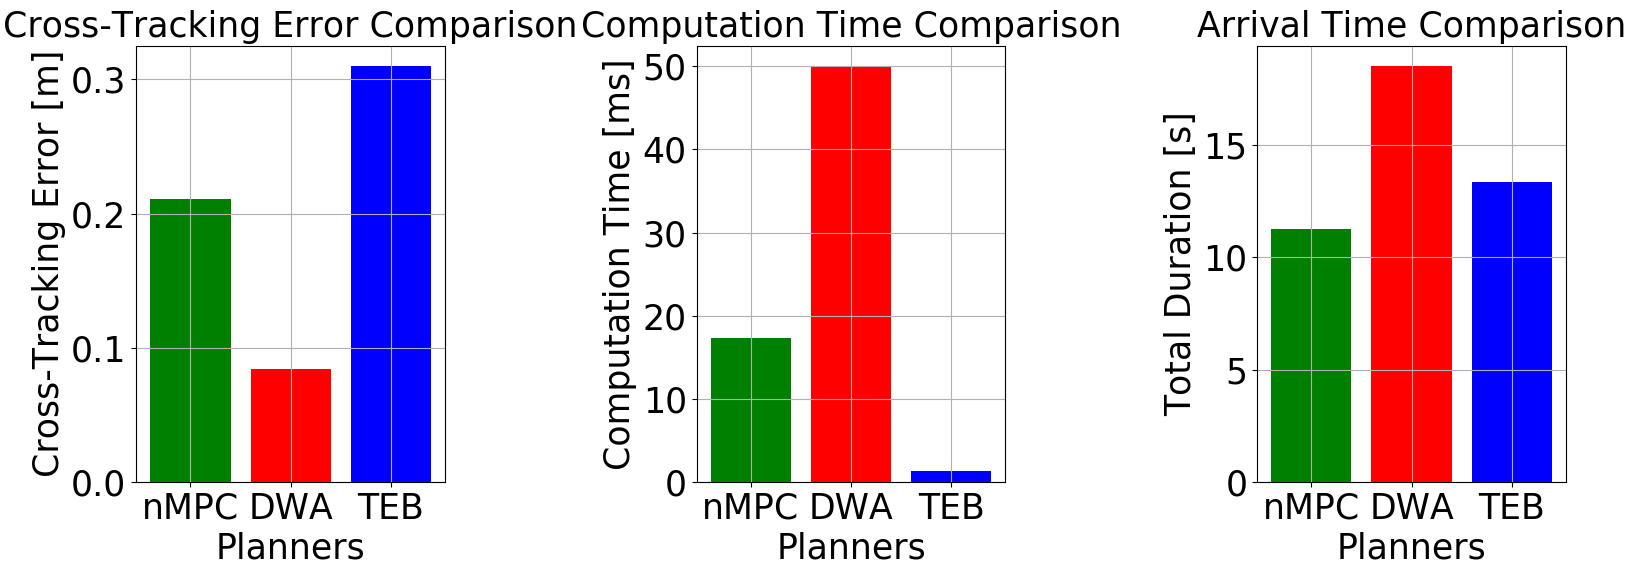
\includegraphics[width=1\columnwidth]{images/nMPC_18_vs_DWA_15_vs_TEB_10.png}
    \caption{Metrics comparison (cross tracking error, computation time, arrival time) for nMPC, DWA, and TEB in Ablation Experiment}
    \label{fig:nMPC_16_vs_DWA_12_vs_TEB_6}
\end{figure}


%%%%%%%%%%%%%%%%%%%%%%%%%%%%%%%%%%%%%%%%%%%%%%%%%%%%%%%%%%%%%%%%%%
\section{Summary and Outlook}

The results demonstrate that the nMPC with soft constraints for obstacle clearance penalization and hard constraints to ensure collision-free paths outperformed the TEB planner in dynamic environments, reducing arrival time by approximately 50 seconds. Compared to DWA, the nMPC was 18 seconds faster in narrow navigation tasks. Although the TEB planner was 2 seconds quicker in very tight passages, the nMPC achieved a lower cross-tracking error relative to the global path. The implemented nMPC offers a flexible local planner, configurable with prediction length, number of obstacles to avoid, and Shi-Tomasi quality level for corner detection. However, further improvements in computation time are necessary to avoid more obstacles without significantly impacting performance. Future work will involve testing the nMPC on real hardware and extending the model to control tracked vehicles using mathematical, data-driven, or hybrid models.

%%%%%%%%%%%%%%%%%%%%%%%%%%%%%%%%%%%%%%%%%%%%%%%%%%%%%%%%%%%%%%%%%%
% Literaturverzeichnis
{\small
\bibliographystyle{IEEEtran}
\bibliography{IEEEabrv,refs}
}


%%%%%%%%%%%%%%%%%%%%%%%%%%%%%%%%%%%%%%%%%%%%%%%%%%%%%%%%%%%%%%%%%%
% End of page 3
\clearpage 

\end{document}